%
% Typography and Publishing - 5th Project
% Ac.Year 2021/2022, Summer Semester
%
% Login xkvace00, Kvacek David
% 1st year BITP, full-time, FIT
% xkvace00@stud.fit.vutbr.cz
%
% Date: 2022-05-05
%

\documentclass{beamer}

\usepackage[czech]{babel}
\usepackage[IL2]{fontenc}
\usepackage[utf8]{inputenc}
\usepackage{amsmath}
\usepackage{graphics}
\usepackage{times}
\usepackage[ruled, czech]{algorithm}
\usepackage{algpseudocode}

\usetheme{Copenhagen}
\usefonttheme[onlylarge]{structurebold}
\setbeamerfont*{frametitle}{size=\normalsize,series=\bfseries}
\setbeamertemplate{navigation symbols}{}
\addtobeamertemplate{navigation symbols}{}{
    \usebeamerfont{footline}
    \usebeamercolor[fg]{footline}
    \hspace{1em}
    \insertframenumber{}\,/\,10
}
\setbeamercolor{footline}{fg=blue}
\setbeamerfont{footline}{series=\bfseries}

\title{Bubble sort}
\subtitle{řadicí algoritmus}
\author{David Kvaček}
\date{\today}

\begin{document}

\begin{frame}
  \titlepage
\end{frame}

\begin{frame}{Motivace}
    \begin{itemize}
        \item Řadicí algoritmy slouží k~třídění určitého typu dat
        \item Jednotlivé položky lze řadit podle hodnoty nebo abecedně
        \item Tyto postupy se dále využívají i~v~jiných oblastech
        \item Řazení může zefektivnit mnohem složitější programy
    \end{itemize}
\end{frame}

\begin{frame}{Princip}
    \begin{itemize}
        \item Bublinkové řazení [známé pod názvem \texttt{bubble sort}] patří mezi nejjednodušší řadicí algoritmy
        \item Hlavní myšlenkou je opakované procházení dat a~porovnávání hodnot sousedících prvků
        \item Špatně seřazené prvky jsou prohozeny (viz Obrázek)
    \end{itemize}
    \pause
    \begin{figure}
        \centering
        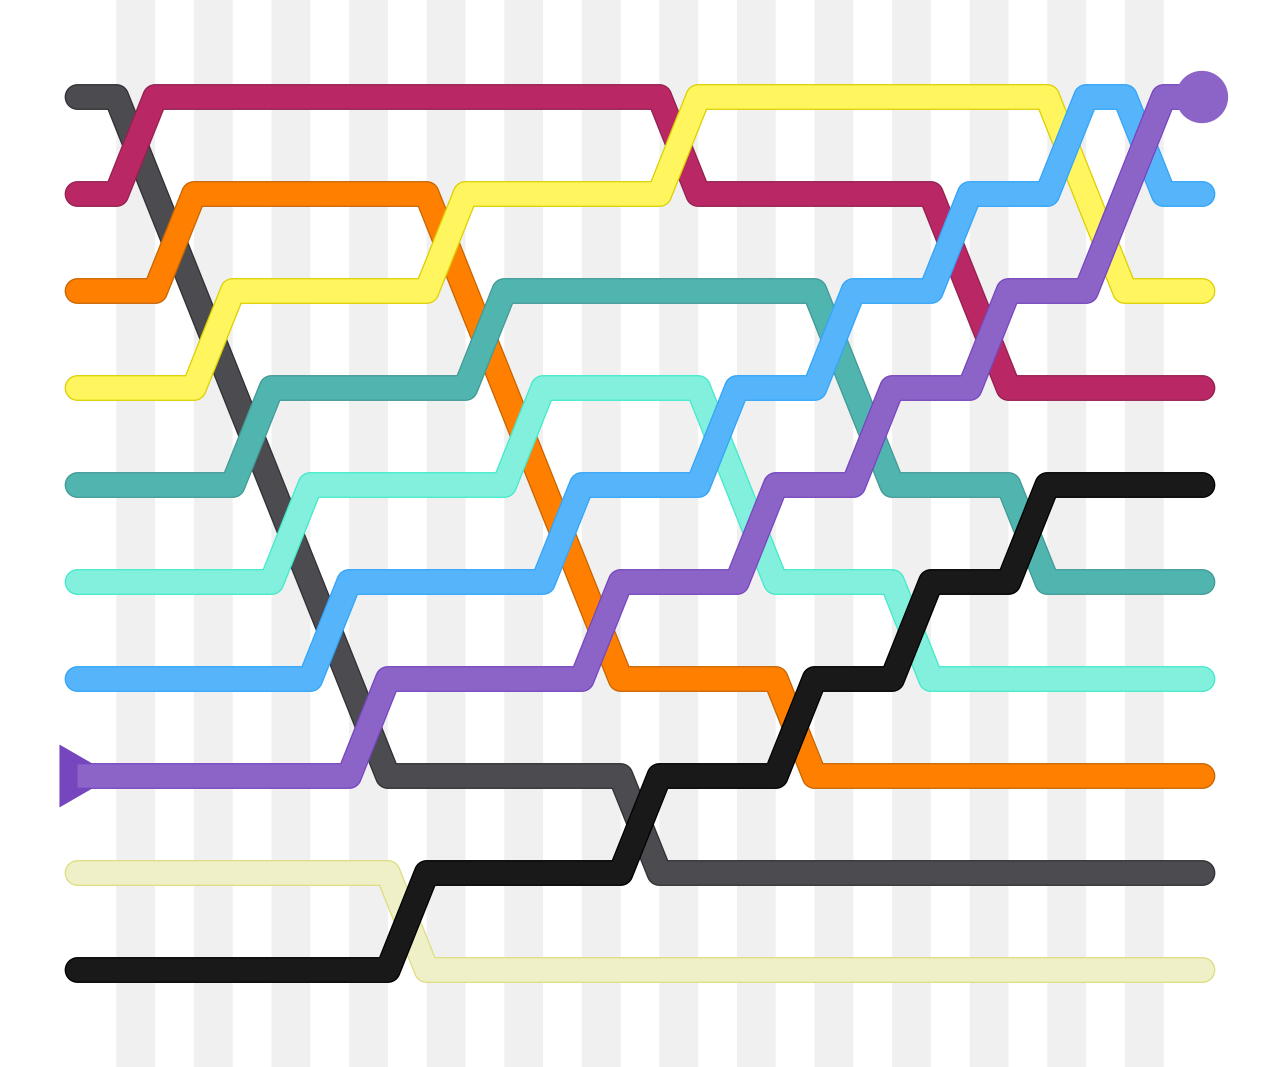
\includegraphics[scale=0.08]{bubble-sort.png}
        \caption{Ukázka třídění pomocí \texttt{bubble sort}}
    \end{figure}
\end{frame}

\begin{frame}{Složitost}
    \begin{itemize}
        \item Časová složitost je u~\texttt{bubble sort} velkou nevýhodou
    \end{itemize}
    \begin{block}{Výkonnost}
        \begin{enumerate}
            \item nejlepší \ldots $O(n)$ \quad [$O(1)$ prohození prvků]
            \item průměr \ldots $O(n^2)$ \quad [$O(n)$ prohození prvků]
            \item nejhorší \ldots $O(n^2)$ \quad [$O(n)$ prohození prvků]
        \end{enumerate}
        \vspace{10pt}
        Poznámka: $n$~značí počet prvků v~poli dat
    \end{block}
\end{frame}

\begin{frame}{Složitost}
    \begin{itemize}
        \item \texttt{Bubble sort} patří k~nejpomalejším řadicím procesům
    \end{itemize}
    \begin{figure}
        \centering
        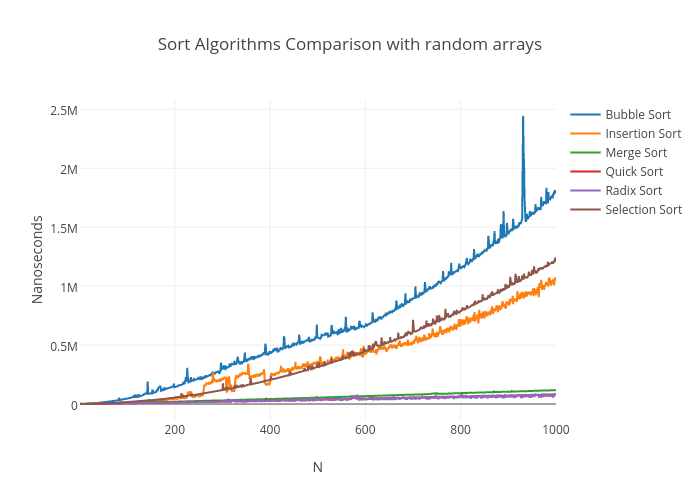
\includegraphics[scale=0.3]{sorting-algorithms.png}
        \caption{Rozdíly ve složitosti řadicích algoritmů}
    \end{figure}
\end{frame}

\begin{frame}{Pseudokód}
    \begin{itemize}
        \item Tento pseudokód řadí hodnoty od nejmenší k~největší
    \end{itemize}
    \begin{algorithm}[H]
        \begin{algorithmic}
            \Function{bubble\_sort}{List *list, int length}
                \For{$n=1$ to $length-1$}
                    \If{$list[n-1] > list[n]$}
                    \\ \qquad \qquad \textbf{swap}($list[n-1]$, $list[n]$)
                    \EndIf
                \EndFor
            \EndFunction
        \end{algorithmic}
    \end{algorithm}
\end{frame}

\begin{frame}{Příklad}
    \begin{figure}
        \centering
        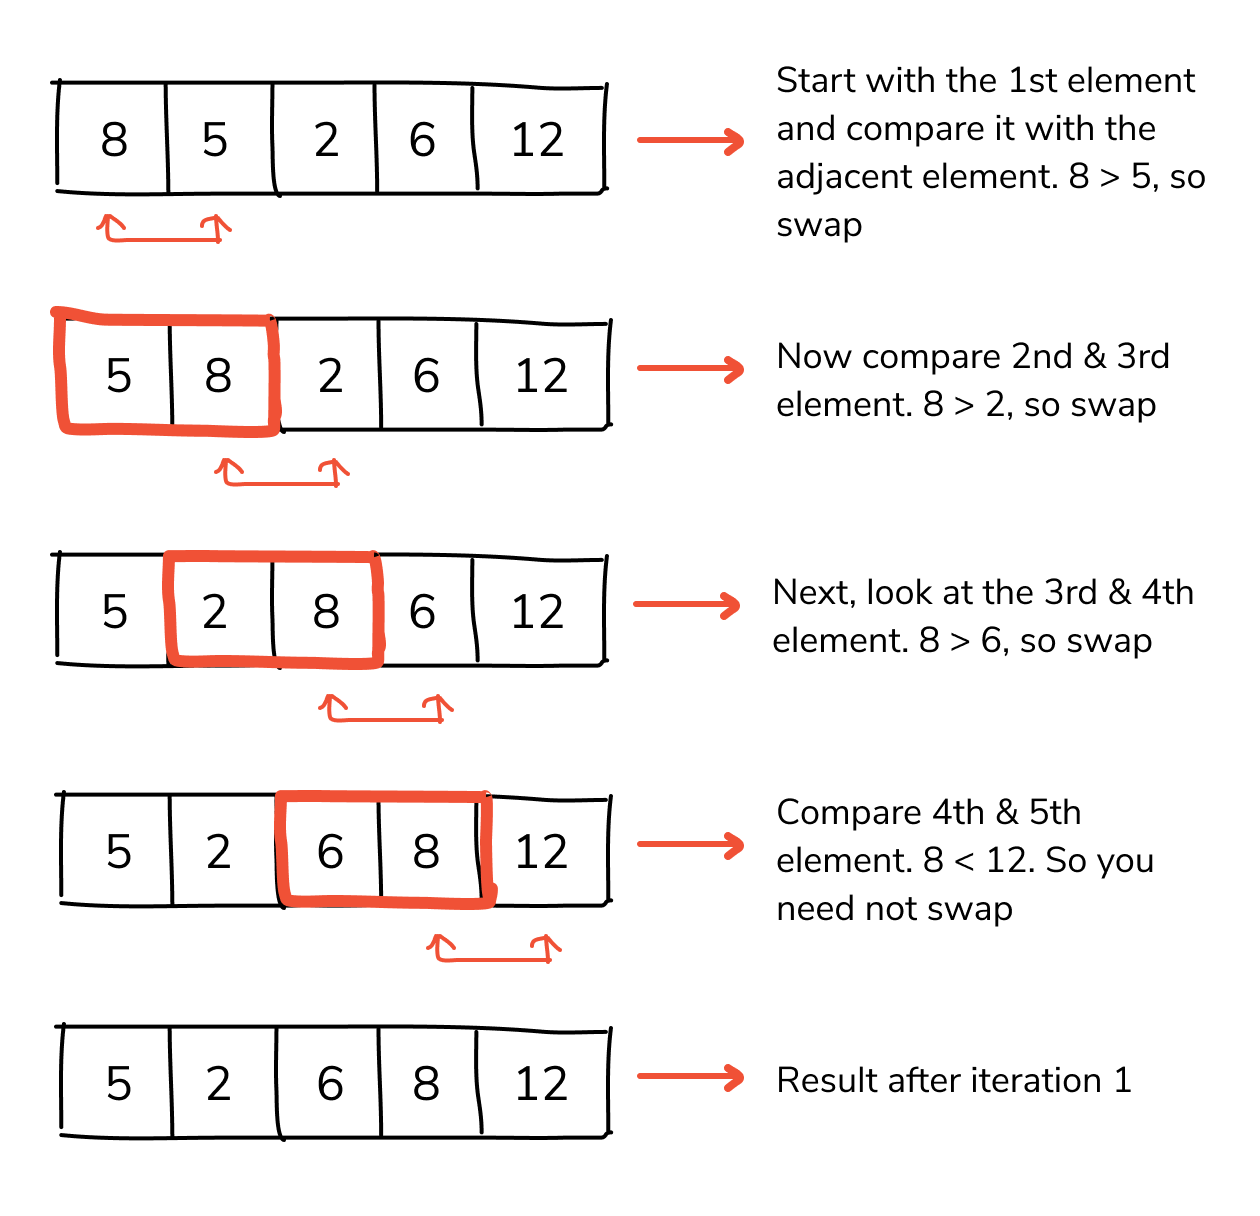
\includegraphics[scale=0.6]{sort-example.png}
        \caption{Ukázka první iterace algoritmu}
    \end{figure}
\end{frame}

\begin{frame}{Shrnutí}
    \pause
    \begin{exampleblock}{Výhody}
        \begin{itemize}
            \item jednoduchý
            \item univerzální
            \item stabilní
        \end{itemize}
    \end{exampleblock}
    \pause
    \begin{alertblock}{Nevýhody}
        \begin{itemize}
            \item pomalý
            \item neefektivní
            \item neoptimalizovaný
        \end{itemize}
    \end{alertblock}
\end{frame}

\begin{frame}{Použité zdroje}
    [Bubble sort]. In: en.Wikipedia.org [online]. 2. května 2022 [cit. 2022-05-04]. Dostupné z: \url{https://en.wikipedia.org/wiki/Bubble_sort}.
    
    [Sort Algorithms Comparison]. In: GitHub.com [online]. 17. ledna 2021 [cit. 2022-05-04]. Dostupné z: \url{https://github.com/MatMercer/Sort-Algorithms-Compare}.
    
    [Bubble Sort in C, C++, Java $|$ FACE Prep]. In: FacePrep.in [online]. 12. března 2020 [cit. 2022-05-04]. Dostupné z: \url{https://www.faceprep.in/c/bubble-sort-in-c/}.
\end{frame}

\begin{frame}{Závěr}
    \centering
    \LARGE
    \textsc{Děkuji za pozornost}
\end{frame}

\end{document}

